\documentclass{beamer}

% !TEX root = ./main.tex
% The above line is a magic comment that tells text editors which file to compile.

\documentclass{beamer}
\usepackage[utf8]{inputenc}
\usepackage{hyperref}
\usepackage{amsmath}
\usepackage{cleveref}
\usepackage{adjustbox}
\usepackage{mathtools}
\usepackage{dsfont}
\usepackage{xcolor}
\usepackage{amsthm}

\usepackage{tikz}
% \usetikzlibrary{arrows.meta}
% \usetikzlibrary{shapes}
% \usetikzlibrary{calc}
% \usetikzlibrary{math}
% \usetikzlibrary{decorations.pathreplacing,calligraphy}
% \usepackage{pgffor}

% \usepackage{algorithm}
% \usepackage{algpseudocode}

\usepackage{macros}
\usepackage{domainmacros}
%%%%%%%%%%
% Beamer %
%%%%%%%%%%

\definecolor{cPurple}{RGB}{124, 0, 133}
\definecolor{cBlue}{RGB}{56, 0, 138}
\definecolor{cRed}{RGB}{180, 0, 60}
\definecolor{cGreen}{RGB}{0, 156, 27}

\usetheme[sectionpage = none, subsectionpage = simple]{metropolis}
\usecolortheme{seahorse}

\usebeamercolor{normal text}
\usebeamercolor{background canvas}

\setbeamercolor{alerted text}{fg=cPurple}

\setbeamertemplate{footline}{%
      \raisebox{8pt}{\makebox[\paperwidth]{\scriptsize \hfill \insertframenumber/\inserttotalframenumber \hspace{5pt}}}}

% \setbeamertemplate{footline}{\raisebox{8pt}{\hfill \insertframenumber/\inserttotalframenumber \hspace{5pt}}}

% \setbeamertemplate{footline}{%
%       \raisebox{8pt}{\makebox[\paperwidth]{\scriptsize \hspace{5pt}  TCS101 \hfill \insertframenumber/\inserttotalframenumber \hfill CC-BY-SA \hspace{5pt}}}}

\beamertemplatenavigationsymbolsempty

\title[RBSR]{Range-Based Set Reconciliation}
\author{Aljoscha Meyer}
\date{}

\begin{document}

\frame{\titlepage}

\begin{frame}{Set Reconciliation}
    \begin{itemize}
        \item set union over a network
        \item between (exactly) two machines
        \item unstructured data
        \item no shared state or history
    \end{itemize}
\end{frame}

\begin{frame}{Trivial Reconciliation}
    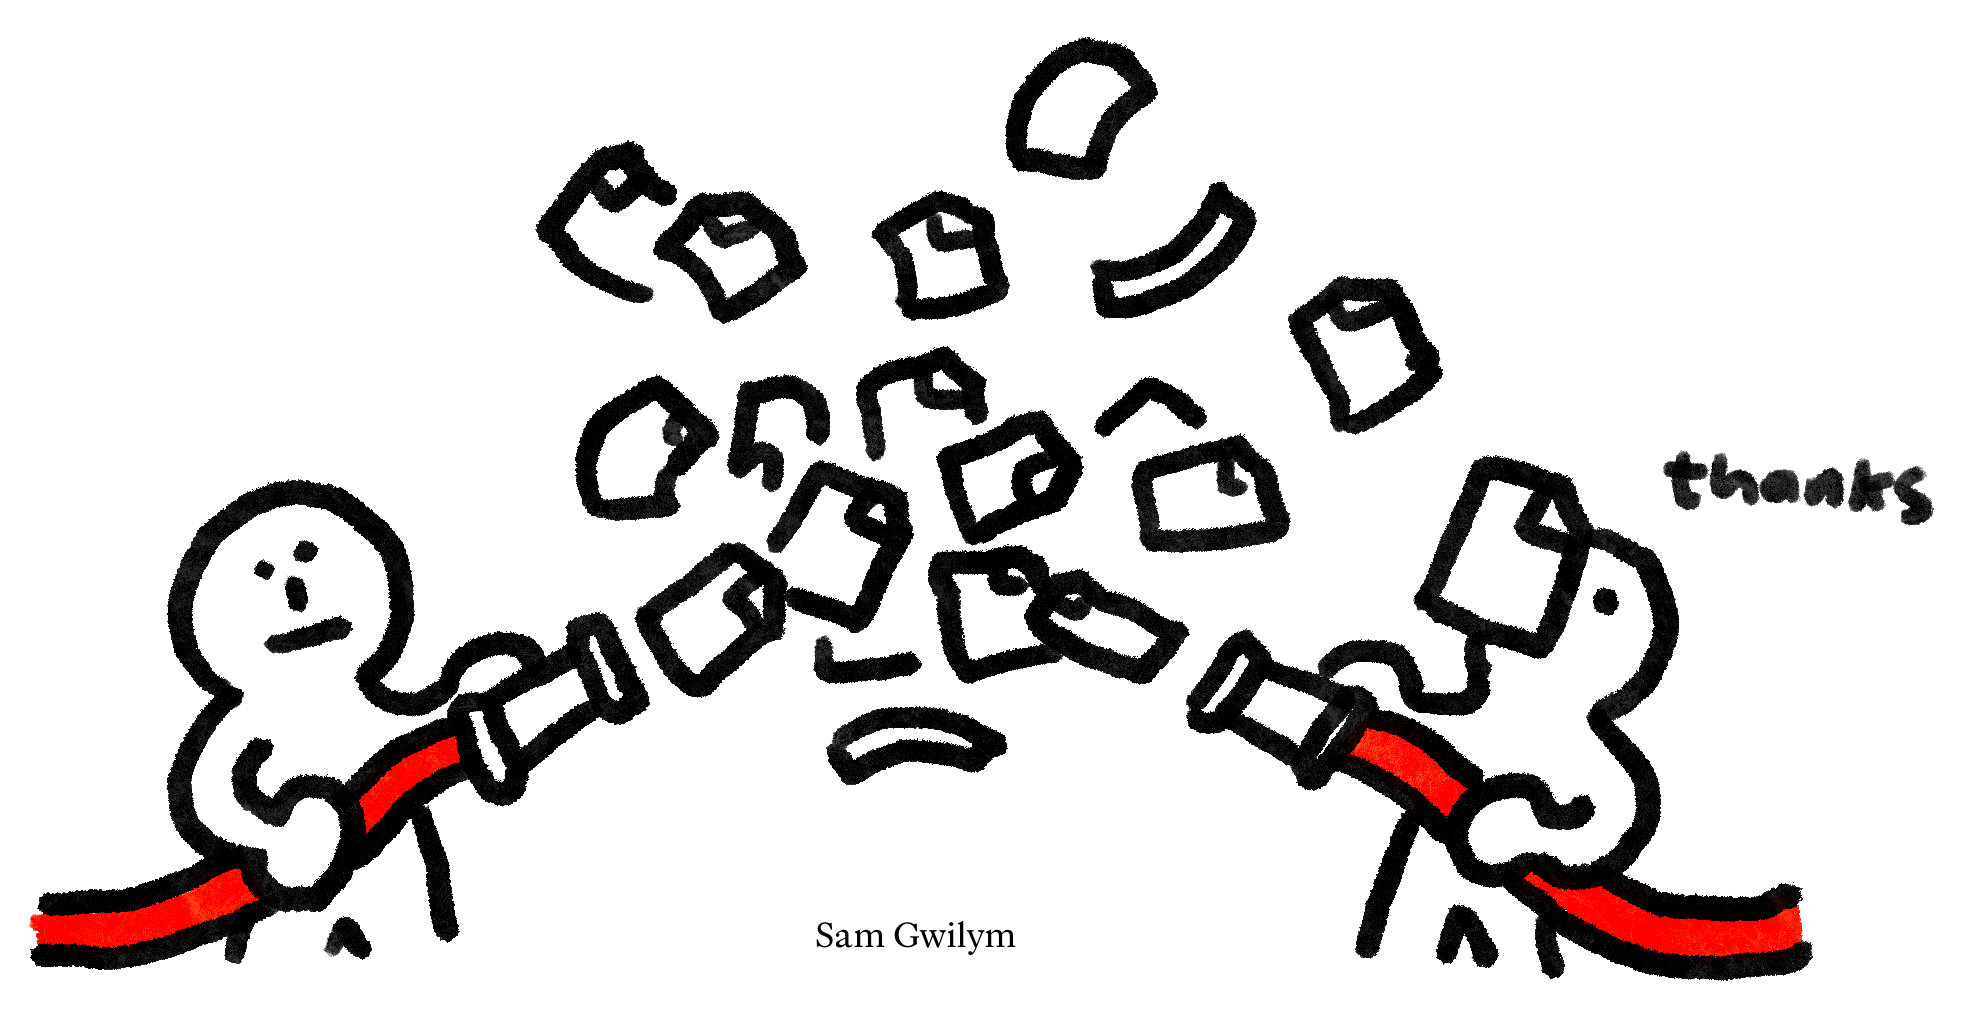
\includegraphics[keepaspectratio=true,width=11.4cm]{trivial_sync.png}
\end{frame}

\begin{frame}{Model and Analysis}
    \begin{itemize}
        \item Alfie and Betty talk over a network
        \item reliable communication, rounds of unit length, unlimited bandwidth
        \item probabilistic solutions \pause
        \item $n$: size of the union
        \item $n_{\triangle}$: size of the symmetric difference
    \end{itemize}
\end{frame}

\begin{frame}{Model and Analysis}
    \begin{itemize}
        \item roundtrips
        \item communicated bytes
        \item computation time per reconciliation session
        \item computation space per reconciliation session
        \item computation time per item
        \item computation space per item
    \end{itemize}
\end{frame}

\begin{frame}{P2P Reconciliation}
    Peer-to-peer systems:
    \begin{itemize}
        \item iterating over local set infeasible
        \item loading local set into memory infeasible
        \item some peers are out to get us
    \end{itemize}

    \pause

    $\implies$ traditional approaches don't work
\end{frame}

\begin{frame}{Reducing Computation Times}
    \begin{itemize}
        \item Step 1: Put a Merkle tree on it
        \item Step 2: ???
        \item Step 3: Profit
    \end{itemize}

    \vfill

    Auvolat, Alex, and François Taïani. "Merkle search trees: Efficient state-based CRDTs in open networks." 2019 38th Symposium on Reliable Distributed Systems (SRDS). IEEE, 2019.
\end{frame}

\begin{frame}{Merkle Trees}
    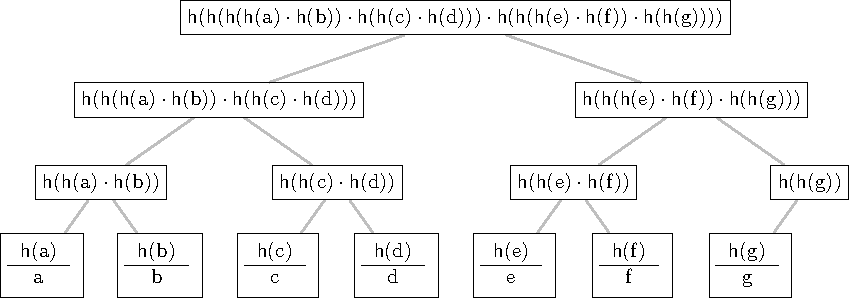
\includegraphics[keepaspectratio=true,width=11.4cm]{merkle1.pdf}
\end{frame}

\begin{frame}{Merkle Trees}
    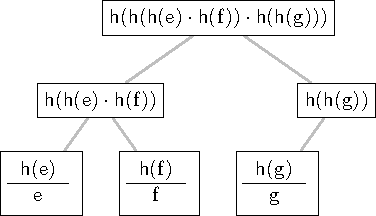
\includegraphics[keepaspectratio=true,width=5cm]{merkle2.pdf}\hfill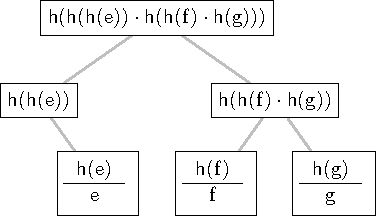
\includegraphics[keepaspectratio=true,width=5cm]{merkle3.pdf}
\end{frame}

\begin{frame}{Merkle Tree Reconciliation}
    \begin{tikzpicture}[xscale=1.6,yscale=0.95][font=\footnotesize]
        \alt<5->{\node (v00) at (0, 0) [treenodeEqual] {\labeledvalue{$147$}{\examplea}};}{\node (v00) at (0, 0) [treenode] {\labeledvalue{$147$}{\examplea}};};
        \alt<5->{\node (v10) at (1, 0) [treenodeUnequal] {\labeledvalue{$821$}{\exampleb}};}{\node (v10) at (1, 0) [treenode] {\labeledvalue{$821$}{\exampleb}};};
        \alt<5->{\node (v30) at (3, 0) [treenodeEqual] {\labeledvalue{$165$}{\exampled}};}{\node (v30) at (3, 0) [treenode] {\labeledvalue{$165$}{\exampled}};};
        \node (v40) at (4, 0) [treenode] {\labeledvalue{$508$}{\examplee}};
        \node (v50) at (5, 0) [treenode] {\labeledvalue{$681$}{\examplef}};
        \node (v60) at (6, 0) [treenode] {\labeledvalue{$570$}{\exampleg}};
    
        \alt<4->{\node (v01) at (0.5, 1) [treenodeUnequal] {$299$};}{\node (v01) at (0.5, 1) [treenode] {$299$};};
        \alt<4->{\node (v11) at (2.5, 1) [treenodeUnequal] {$212$};}{\node (v11) at (2.5, 1) [treenode] {$212$};};
        \node (v21) at (4.5, 1) [treenode] {$996$};
        \node (v31) at (6.5, 1) [treenode] {$974$};
    
        \alt<3->{\node (v02) at (1.5, 2) [treenodeUnequal] {$772$};}{\node (v02) at (1.5, 2) [treenode] {$772$};};
        \alt<3->{\node (v12) at (5.5, 2) [treenodeEqual] {$336$};}{\node (v12) at (5.5, 2) [treenode] {$336$};};
    
        \alt<2->{\node (v03) at (3.5, 3) [treenodeUnequal] {$242$};}{\node (v03) at (3.5, 3) [treenode] {$242$};};
    
        \draw (v00) edge[edge] (v01);
        \draw (v10) edge[edge] (v01);
        \draw (v30) edge[edge] (v11);
        \draw (v40) edge[edge] (v21);
        \draw (v50) edge[edge] (v21);
        \draw (v60) edge[edge] (v31);
    
        \draw (v01) edge[edge] (v02);
        \draw (v11) edge[edge] (v02);
        \draw (v21) edge[edge] (v12);
        \draw (v31) edge[edge] (v12);
        
        \draw (v02) edge[edge] (v03);
        \draw (v12) edge[edge] (v03);
    \end{tikzpicture}

    \begin{tikzpicture}[xscale=1.6,yscale=0.95][font=\footnotesize]
        \alt<5->{\node (v00) at (0, 0) [treenodeEqual] {\labeledvalue{$147$}{\examplea}};}{\node (v00) at (0, 0) [treenode] {\labeledvalue{$147$}{\examplea}};};
        \alt<5->{\node (v20) at (2, 0) [treenodeUnequal] {\labeledvalue{$260$}{\examplec}};}{\node (v20) at (2, 0) [treenode] {\labeledvalue{$260$}{\examplec}};};
        \alt<5->{\node (v30) at (3, 0) [treenodeEqual] {\labeledvalue{$165$}{\exampled}};}{\node (v30) at (3, 0) [treenode] {\labeledvalue{$165$}{\exampled}};};
        \node (v40) at (4, 0) [treenode] {\labeledvalue{$508$}{\examplee}};
        \node (v50) at (5, 0) [treenode] {\labeledvalue{$681$}{\examplef}};
        \node (v60) at (6, 0) [treenode] {\labeledvalue{$570$}{\exampleg}};
    
        \alt<4->{\node (v01) at (0.5, 1) [treenodeUnequal] {$089$};}{\node (v01) at (0.5, 1) [treenode] {$089$};};
        \alt<4->{\node (v11) at (2.5, 1) [treenodeUnequal] {$602$};}{\node (v11) at (2.5, 1) [treenode] {$602$};};
        \node (v21) at (4.5, 1) [treenode] {$996$};
        \node (v31) at (6.5, 1) [treenode] {$974$};
    
        \alt<3->{\node (v02) at (1.5, 2) [treenodeUnequal] {$446$};}{\node (v02) at (1.5, 2) [treenode] {$446$};};
        \alt<3->{\node (v12) at (5.5, 2) [treenodeEqual] {$336$};}{\node (v12) at (5.5, 2) [treenode] {$336$};};
    
        \alt<2->{\node (v03) at (3.5, 3) [treenodeUnequal] {$571$};}{\node (v03) at (3.5, 3) [treenode] {$571$};};
    
        \draw (v00) edge[edge] (v01);
        \draw (v20) edge[edge] (v11);
        \draw (v30) edge[edge] (v11);
        \draw (v40) edge[edge] (v21);
        \draw (v50) edge[edge] (v21);
        \draw (v60) edge[edge] (v31);
    
        \draw (v01) edge[edge] (v02);
        \draw (v11) edge[edge] (v02);
        \draw (v21) edge[edge] (v12);
        \draw (v31) edge[edge] (v12);
        
        \draw (v02) edge[edge] (v03);
        \draw (v12) edge[edge] (v03);
    \end{tikzpicture}
\end{frame}

\begin{frame}{Merkle Tree Reconciliation}
    \begin{itemize}
        \item inflexible data representation
        \item inacceptable worst-case complexity \begin{itemize}
            \item remember, some peers are out to get us
        \end{itemize}
    \end{itemize}
\end{frame}

\begin{frame}{Range-Based Set Reconciliation}
    $X_{\alpha} \defeq \{\exampleb, \examplec, \exampled, \examplee, \examplef, \exampleh \}$
    \hfill
    $X_{\beta} \defeq \{\examplea, \examplee, \examplef, \exampleg\}$
    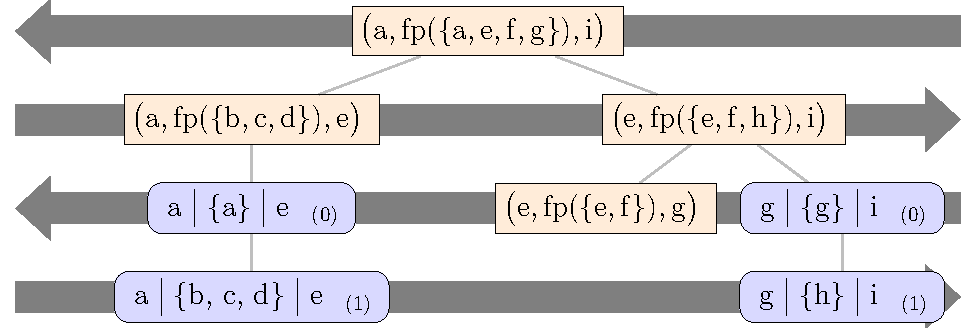
\includegraphics[keepaspectratio=true,width=11.4cm]{examplerun.pdf}

    % \item hence relax to logarithmic number of rounds
    % \item divide-and-conquer -> explain rbsr
    % \item complexity analysis
\end{frame}

\begin{frame}{Some Nice Properties}
    \begin{itemize}
        \item reasonably efficient: $\complexity{\min(n_{\triangle} \cdot \log(n), n)}$ bytes communication, $\complexity{1}$ working memory
        \item can interpolate toward trivial
        \item arbitrary recursion anchor protocols
        \item arbitrary partition techniques \pause
        \item but: linear computation times
    \end{itemize}
\end{frame}

\begin{frame}{Order-Statistic Trees\only<2->{ $[\examplec, \examplei)$}}
    \begin{tikzpicture}[xscale=0.95,yscale=1.6][font=\footnotesize]
        \pgfdeclarelayer{background}
        \pgfdeclarelayer{foreground}
        \pgfsetlayers{background,main,foreground}

        \begin{pgfonlayer}{main}
            \node (v00) at (0, 0) [treenodeSmall] {\labeledvalue{$1$}{\examplea}};
            \node (v10) at (1, 0) [treenodeSmall] {\labeledvalue{$1$}{\exampleb}};
            \node (v20) at (2, 0) [treenodeSmall] {\labeledvalue{$1$}{\examplec}};
            \node (v30) at (3, 0) [treenodeSmall] {\labeledvalue{$1$}{\exampled}};
            \node (v40) at (4, 0) [treenodeSmall] {\labeledvalue{$1$}{\examplee}};
            \node (v50) at (5, 0) [treenodeSmall] {\labeledvalue{$1$}{\examplef}};
            \node (v60) at (6, 0) [treenodeSmall] {\labeledvalue{$1$}{\exampleg}};
            \node (v80) at (8, 0) [treenodeSmall] {\labeledvalue{$1$}{\exampleh}};
            % \node (v90) at (9, 0) [treenodeSmall] {\labeledvalue{$1$}{\examplei}};
            \node (v100) at (10, 0) [treenodeSmall] {\labeledvalue{$1$}{\examplei}};
            \node (v110) at (11, 0) [treenodeSmall] {\labeledvalue{$1$}{\examplej}};
        
            \node (v01) at (0.5, 1) [treenode] {$2$};
            \node (v11) at (2.5, 1) [treenode] {$2$};
            \node (v21) at (4.5, 1) [treenode] {$2$};
            \node (v31) at (6, 1) [treenode] {$1$};
            \node (v41) at (8, 1) [treenode] {$1$};
            \node (v51) at (10.5, 1) [treenode] {$2$};
        
            \node (v02) at (1.5, 2) [treenode] {$4$};
            \node (v12) at (5.5, 2) [treenode] {$3$};
            \node (v22) at (9.5, 2) [treenode] {$3$};
        
            \node (v03) at (3.5, 3) [treenode] {$7$};
            \node (v13) at (9.5, 3) [treenode] {$7$};

            \node (v04) at (7.5, 4) [treenode] {$14$};
        
            \draw (v00) edge[edge] (v01);
            \draw (v10) edge[edge] (v01);
            \draw (v20) edge[edge] (v11);
            \draw (v30) edge[edge] (v11);
            \draw (v40) edge[edge] (v21);
            \draw (v50) edge[edge] (v21);
            \draw (v60) edge[edge] (v31);
            \draw (v80) edge[edge] (v41);
            \draw (v100) edge[edge] (v51);
            \draw (v110) edge[edge] (v51);
        
            \draw (v01) edge[edge] (v02);
            \draw (v11) edge[edge] (v02);
            \draw (v21) edge[edge] (v12);
            \draw (v31) edge[edge] (v12);
            \draw (v41) edge[edge] (v22);
            \draw (v51) edge[edge] (v22);
            
            \draw (v02) edge[edge] (v03);
            \draw (v12) edge[edge] (v03);
            \draw (v22) edge[edge] (v13);

            \draw (v03) edge[edge] (v04);
            \draw (v13) edge[edge] (v04);
        \end{pgfonlayer}

        \begin{pgfonlayer}{foreground}
            \only<2->{
                \draw[draw=black, fill=black, opacity=0.6] (-0.5,-0.5) rectangle (1.5,4.5);
                \draw[draw=black, fill=black, opacity=0.6] (9.5,-0.5) rectangle (11.5,4.5);
            }
        \end{pgfonlayer}

        \begin{pgfonlayer}{background}
            \begin{scope}[transparency group, opacity=0.4]
                \only<4->{
                    \draw[draw=orange, fill=orange] (7.1,3.75) rectangle ++(0.8,0.5);
                }

                \only<5->{
                    \draw[orange,line width=11pt,rounded corners=0.1em,line cap=round] (v04.center) -- (v03.center) -- (v02.center) -- (v11.center);
                    \draw[orange,line width=11pt,rounded corners=1em,line cap=round] (v04.center) -- (v03.center) -- (v02.center) -- (v11.center);

                    \draw[orange,line width=11pt,rounded corners=0.1em,line cap=round] (v04.center) -- (v13.center) -- (v22.center) -- (v41.center);
                    \draw[orange,line width=11pt,rounded corners=1em,line cap=round] (v04.center) -- (v13.center) -- (v22.center) -- (v41.center);
                }                

                \only<3->{
                    \draw[draw=violet, fill=violet] (2.1,0.75) rectangle ++(0.8,0.5);
                    \draw[draw=violet, fill=violet] (5.1,1.75) rectangle ++(0.8,0.5);
                    \draw[draw=violet, fill=violet] (7.6,0.75) rectangle ++(0.8,0.5);
                }
            \end{scope}
        \end{pgfonlayer}
    \end{tikzpicture}
\end{frame}

\begin{frame}{Monoid Trees}
    \begin{itemize}
        \item set of labels: $\N$
        \item binary associative function: $+$
        \item neutral element: $0$\pause
        \item lifting into the monoid: $\lambda x.1$
    \end{itemize}

    \begin{itemize}
        \item<3-> set of labels: $\set{n \st 0 <= n < 2^{256} - 1}$
        \item<4-> binary associative function: xor
        \item<4-> neutral element: $0$
        \item<3-> lifting into the monoid: sha256
    \end{itemize}
\end{frame}

\begin{frame}{Advantages}
    \begin{itemize}
        \item solid worst-case communication complexity
        \item implementation independence
    \end{itemize}
\end{frame}

\begin{frame}{Alternative Datastructures}
    \begin{tikzpicture}[xscale=1.5,yscale=1.6][font=\footnotesize]
        \pgfdeclarelayer{background}
        \pgfdeclarelayer{foreground}
        \pgfsetlayers{background,main,foreground}

        \begin{pgfonlayer}{main}
            \node (v00) at (0, 0) [treenodeSmall] {\labeledvalue{$1$}{\examplea}};
            \node (v10) at (1, 0) [treenodeSmall] {\labeledvalue{$1$}{\examplec}};
            \node (v20) at (2, 0) [treenodeSmall] {\labeledvalue{$1$}{\examplee}};
            \node (v30) at (3, 0) [treenodeSmall] {\labeledvalue{$1$}{\exampleg}};
            \node (v40) at (4, 0) [treenodeSmall] {\labeledvalue{$1$}{\examplei}};
            \node (v50) at (5, 0) [treenodeSmall] {\labeledvalue{$1$}{\examplek}};
            \node (v60) at (6, 0) [treenodeSmall] {\labeledvalue{$1$}{\examplem}};
        
            \node (v01) at (0.5, 1) [treenodeSmall] {\labeledvalue{$3$}{\exampleb}};
            \node (v11) at (2.5, 1) [treenodeSmall] {\labeledvalue{$3$}{\examplef}};
            \node (v21) at (4.5, 1) [treenodeSmall] {\labeledvalue{$3$}{\examplej}};
            \node (v31) at (6.5, 1) [treenodeSmall] {\labeledvalue{$2$}{\examplen}};
        
            \node (v02) at (1.5, 2) [treenodeSmall] {\labeledvalue{$7$}{\exampled}};
            \node (v12) at (5.5, 2) [treenodeSmall] {\labeledvalue{$6$}{\examplel}};
        
            \node (v03) at (3.5, 3) [treenode] {\labeledvalue{$14$}{\exampleh}};
        
            \draw (v00) edge[edge] (v01);
            \draw (v10) edge[edge] (v01);
            \draw (v20) edge[edge] (v11);
            \draw (v30) edge[edge] (v11);
            \draw (v40) edge[edge] (v21);
            \draw (v50) edge[edge] (v21);
            \draw (v60) edge[edge] (v31);
        
            \draw (v01) edge[edge] (v02);
            \draw (v11) edge[edge] (v02);
            \draw (v21) edge[edge] (v12);
            \draw (v31) edge[edge] (v12);
            
            \draw (v02) edge[edge] (v03);
            \draw (v12) edge[edge] (v03);
        \end{pgfonlayer}

        \begin{pgfonlayer}{foreground}
            \only<2->{
                \draw[draw=black, fill=black, opacity=0.6] (-0.5,-0.5) rectangle (0.8,4.5);
                \draw[draw=black, fill=black, opacity=0.6] (4.8,-0.5) rectangle (8.5,4.5);
            }
        % \end{pgfonlayer}

        % \begin{pgfonlayer}{background}
            \begin{scope}[transparency group, opacity=0.3]
                \only<5->{
                    \draw[orange,line width=11pt,rounded corners=0.1em,line cap=round] (v03.center) -- (v02.center) -- (v01.center) -- (v10.center);
                    \draw[orange,line width=11pt,rounded corners=1em,line cap=round] (v03.center) -- (v02.center) -- (v01.center) -- (v10.center);
                    \draw[orange,line width=11pt,rounded corners=0.1em,line cap=round] (v03.center) -- (v12.center) -- (v21.center);
                    \draw[orange,line width=11pt,rounded corners=1em,line cap=round] (v03.center) -- (v12.center) -- (v21.center);
                }                

                \only<3->{
                    \draw[draw=violet, fill=violet] (0.7,-0.05) rectangle ++(0.6,0.5);
                    \draw[draw=violet, fill=violet] (2.2,0.95) rectangle ++(0.6,0.5);
                    \draw[draw=violet, fill=violet] (3.7,-0.05) rectangle ++(0.6,0.5);
                }

                \only<4->{
                    \draw[draw=blue, fill=blue] (1.2,1.6) rectangle ++(0.6,0.42);
                    \draw[draw=blue, fill=blue] (3.1,2.63) rectangle ++(0.8,0.42);
                    \draw[draw=blue, fill=blue] (4.2,0.6) rectangle ++(0.6,0.42);
                }
            \end{scope}
        \end{pgfonlayer}
    \end{tikzpicture}
\end{frame}

\begin{frame}{Successive Ranges}
    
\end{frame}


\begin{itemize}
    \item malicious adversaries: active vs passive
    \item even passive finds collisions in relatively small sets
    \item but: collision must actually affect a session -> brittle, and randomization ftw
    \item But what if there are many collisions? -> collision-resistant hash functions
\end{itemize}

\begin{itemize}
    \item must always lift into the monoid with a secure hash function. Interesting part is the selection of the monoid
    \item bellare: xor, addition, multiplication, vectorized addition (lattices)
    \item multiset homomorphic hashing adds rsa and elliptic curves
    \item we are weaker: homomorphism-flavored characterization
    \item in particular, no need for commutativity (because we use search trees) -> matrix multiplication -> cayley hashes
    \item Don't know anything else, but cayley still has unnecesary structure, as we do not need inverses
\end{itemize}

\begin{itemize}
    \item conclusion: first non-trivial reconciliation algorithm to work in resource-constrained settings and adversarial environments
    \item also: comparatively simple -> had multiple open source developers reach out to me
\end{itemize}
% \end{frame}

\end{document}
